\documentclass[a4paper,14pt]{extarticle} % Используем extarticle для поддержки шрифта 14
\usepackage[utf8]{inputenc}
\usepackage[T2A]{fontenc}
\usepackage[russian]{babel}
\usepackage{amsmath}
\usepackage{amssymb}
\usepackage{graphicx}
\usepackage[left=3cm,right=2cm,top=2cm,bottom=2cm]{geometry}
\linespread{1.5}

\begin{document}

\begin{titlepage}
    \begin{center}
        \large
        Министерство науки и высшего образования Российской Федерации \\
        Санкт-Петербургский государственный электротехнический университет \\
        \textbf{«ЛЭТИ» им. В.И. Ульянова (Ленина)} \\
        Кафедра систем автоматического управления

        \vfill

        \textbf{Реферат} \\
        по дисциплине \\
        \textbf{«Нелинейное адаптивное управление в технических системах»}

        \vfill

        Студент группы 9492 \hfill Викторов А.Д. \\
        Преподаватель \hfill Путов В.В.

        \vfill
        Санкт-Петербург \\
        2024
    \end{center}
\end{titlepage}

\setcounter{page}{2}
\tableofcontents

\newpage
\begin{abstract}
    В данной работе рассматриваются методы управления нелинейными неопределенными объектами, когда нарушаются условия согласования системы. Основное внимание уделяется методу робастного обхода интегратора, а также синтезу управления на основе двухшаговой итеративной процедуры. Приведены основные подходы и решения, которые помогают обеспечить устойчивость системы и достичь заданных целей управления в условиях неопределенности. Описаны математические модели, необходимые для реализации данных методов, а также предложены примеры их применения.
\end{abstract}

\newpage
\section{Введение}
Управление нелинейными неопределенными объектами представляет собой одну из наиболее сложных задач в теории автоматического управления. В реальных системах могут возникать различные неопределенности, связанные как с внешними воздействиями, так и с недостаточной информацией о динамике объекта. Особенно сложными становятся задачи управления, когда нарушаются условия согласования. Одним из подходов, позволяющих справиться с этими проблемами, является метод робастного обхода интегратора, который будет рассмотрен в данной работе.

\newpage
\section{Проблема управления при нарушении условий согласования}
Для управления нелинейными системами требуется выполнение условий согласования, которые гарантируют возможность синтеза эффективного управления. Однако в реальных условиях данные предположения могут не выполняться. Это приводит к необходимости разработки методов, которые учитывают неопределенности и позволяют стабилизировать систему.

\subsection{Определение условий согласования}
Условия согласования определяют взаимосвязь между входами и выходами системы, которая обеспечивает возможность существования управляющего воздействия, стабилизирующего объект. Для нелинейной системы вида:
\begin{equation}
    \dot{x} = f(x) + g(x)u,
\end{equation}
где \(x \in \mathbb{R}^n\) — вектор состояния, \(u \in \mathbb{R}^m\) — вектор управления, \(f(x)\) и \(g(x)\) — нелинейные функции, описывающие динамику системы, условия согласования определяют, что система должна быть управляемой для всех \(x\). Нарушение условий согласования может приводить к невозможности прямого применения методов линейной теории управления.

\newpage
\section{Метод робастного обхода интегратора}
Метод робастного обхода интегратора основан на введении дополнительных коррекций в управление, которые позволяют компенсировать неопределенности и нарушения условий согласования. Этот подход особенно полезен в тех случаях, когда точная модель системы неизвестна или параметры системы изменяются во времени.

\begin{figure}[h]
\center{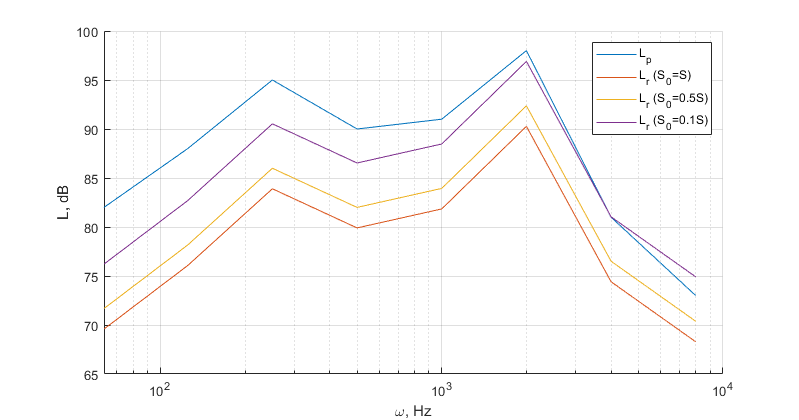
\includegraphics[width=1\linewidth]{1.png}}
\caption{Эквивалентное представление системы.}
\label{1.png:image}
\end{figure}

\subsection{Основные этапы метода}
Метод робастного обхода интегратора включает несколько ключевых шагов:
\begin{enumerate}
    \item Формулировка задачи управления с учетом неопределенностей:
    \begin{equation}
        \dot{x} = f(x) + g(x)(u + \Delta u),
    \end{equation}
    где \(\Delta u\) — робастная корректировка управления.
    \item Определение структуры управления с применением робастных корректировок:
    \begin{equation}
        u = -Kx - \alpha(x),
    \end{equation}
    где \(K\) — матрица обратной связи, а \(\alpha(x)\) — корректирующая функция, компенсирующая влияние нелинейностей и неопределенностей.
    \item Применение итеративных методов для поиска оптимального решения, где корректировка проводится до достижения приемлемого уровня устойчивости.
\end{enumerate}

\subsection{Вывод устойчивости системы}
Для оценки устойчивости системы после применения робастного обхода интегратора используется функция Ляпунова \(V(x)\):
\begin{equation}
    V(x) = \frac{1}{2}x^T P x,
\end{equation}
где \(P\) — положительно определенная матрица. Производная функции Ляпунова должна удовлетворять условию:
\begin{equation}
    \dot{V}(x) = x^T P \dot{x} \leq -\alpha \|x\|^2,
\end{equation}
где \(\alpha > 0\). Это условие гарантирует асимптотическую устойчивость системы.

\newpage
\section{Двухшаговая итеративная процедура синтеза}
Одной из эффективных техник для синтеза управления в условиях неопределенности является двухшаговая итеративная процедура. В этой процедуре на первом этапе происходит начальная оценка параметров системы, а на втором этапе осуществляется корректировка управления с учетом полученных данных.

\subsection{Первый шаг: оценка состояния системы}
На первом этапе процедуры проводится анализ состояния системы и оценка параметров, которые могут быть подвержены неопределенности. Используется метод наблюдателя состояния, описываемый уравнением:
\begin{equation}
    \hat{x} = f(\hat{x}) + g(\hat{x})u + L(y - \hat{y}),
\end{equation}
где \(\hat{x}\) — оценка состояния, \(y\) — измеряемый выход системы, \(L\) — матрица наблюдателя. Этот шаг позволяет приблизительно оценить поведение системы и определить начальные условия для дальнейшего синтеза управления.

\subsection{Второй шаг: корректировка управления}
На втором этапе управление корректируется с использованием робастных методов для минимизации влияния неопределенностей:
\begin{equation}
    u_{k+1} = u_k + \Delta u_k,
\end{equation}
где \(\Delta u_k\) — корректировка на \(k\)-м шаге, рассчитываемая на основе текущего состояния \(\hat{x}_k\) и оценок параметров. Процесс итеративно повторяется до достижения заданного критерия устойчивости:
\begin{equation}
    \|x - \hat{x}\| < \varepsilon,
\end{equation}
где \(\varepsilon\) — допустимая погрешность.

\newpage
\section{Заключение}
Методы управления нелинейными неопределенными объектами требуют разработки сложных алгоритмов, которые учитывают неопределенности и нарушения согласования. Метод робастного обхода интегратора и двухшаговая итеративная процедура синтеза представляют собой эффективные подходы к решению данных задач, обеспечивая устойчивость и надежность управления в реальных системах. Эти методы находят применение в широком спектре задач, начиная от управления роботизированными системами и заканчивая управлением технологическими процессами, где важно учитывать изменяющиеся условия и неопределенность параметров.

\end{document}